\section{Math-in-the-Middle Interoperability}\label{sec:mitm}

To build a VRE toolkit from open-source (or open-API\footnote{It turns out that it is
  sufficient to have a well-documented API that gives access to the internal
  (mathematical) data structures and functionality, so closed-source systems can also be
  part of the MitM paradigm if they do.}) systems, we need a joint user interface -- the
OpenDreamKit project adopts Jupyter~\cite{jupyter-project:on} and active
documents~\cite{KohDavGin:psewads11} -- and an interoperability layer that allows to pass
problems and results between the disparate systems. 

For the latter -- and that is the topic of this paper -- we need a way to mediate between
the interaction layers of the respective systems. Generally, mathematical software systems
have apply operations on mathematical objects, which can be expressed as domain-specific
constructors to primitive objects like numbers. The results of these operations are again
such objects. If we abstract from issues of surface syntax -- which we can by assuming
that the systems use a standard like OpenMath~\cite{BusCapCar:2oms04}, the interface
languages differ in their vocabularies -- the operations and constructors. The difficulty
in the translation of objects and functionalities between systems is to align the
respective vocabularies: constructors of system $A$ can be operations in $B$ and vice
versa, even when $A$ and $B$ deal with the mathematically ``same objects'', these may be
constructed differently, and even if $A$ and $B$ share constructors and operations, these
can differ in argument order/number, types, etc.

\subsection{The MitM Paradigm}\label{sec:mitm:recap}

Obviously, a P2P translation regime ($n^2$ translations between all systems) is already
intractable for the systems in the OpenDreamKit project (more than a dozen), and a
``industry standard'' regime where one interaction language is declared as a ``standard''
is infeasible, since no system subsumes the others in terms of coverage -- apart from the
political problems such a standardization would induce. Instead we have proposed the
``Math-in-the-Middle'' (MitM) approach, where we use ``mathematical knowledge'' as an
independent mediating vocabulary, and all system vocabularies are aligned to that. After
all, the mathematics behind the systems is published using this vocabulary.

\begin{wrapfigure}r{4.3cm}\vspace*{-2em}
  \tikzinput{mistargraph}\vspace*{-1em}
  \caption{MitM Paradigm}\label{fig:mitm}\vspace*{-1.5em}
\end{wrapfigure}
Figure~\ref{fig:mitm} shows the setup of the MitM paradigm -- see~\cite{DehKohKon:iop16}
for details. In the center, we have the \textbf{MitM Ontology}, which is a modular
flexiformalization of the mathematical knowledge behind the systems $A$ to $H$ as a theory
graph in the OMDoc/MMT Format~\cite{Kohlhase:OMDoc1.2,RabKoh:WSMSML13,uniformal:on}. For
each of the systems $A$ to $H$, we generate a theory graph \textbf{API Content
  Dictionaries}\footnote{In~\cite{DehKohKon:iop16} we had called these ``interface
  theories'', but we would like to reserve this term for certain theories in the MitM
  ontology.}\ednote{MK: we may want to change this term before we submit; let's discuss!}
in OMDoc/MMT which is aligned with the corresponding symbols in the MitM ontology. As the
API CDs and the MitM Ontology are both in OMDoc/MMT -- inside the cloud in
Figure~\ref{fig:mitm} -- we can make use of \textbf{OMDoc/MMT
  alignments}~\cite{MueGauKal:cacfms17} which have been developed in the meantime for the
MitM alignment relation.\ednote{MK: talk about interface theories somewhere below}

\subsection{OpenMath System Dialects and Alignment-based Translation}\label{sec:mitm:dialect}

Given the collection $s$ of API CDs of a system $S$ (see section~\ref{sec:apit} for
examples), we can express all the API objects in the interface language of $S$ as OpenMath
objects that only use symbols from $s$. 
We call this language the \textbf{OpenMath system dialect} for $S$ and refer to OM objects in this language as $S$-objects. 
Given an OpenMath \textbf{phrasebook}, i.e. an OpenMath interface that allows to serialize
and parse all API objects of $S$ as OpenMath objects in the system dialect of $S$ (see~\cite[Section
1.5]{BusCapCar:2oms04}).

Note that as we have included the operations in the system API CDs of $S$, we can express all the functionality of $S$ in terms of OpenMath objects: if we want GAP to compute the normalizer of a group $G$, we can express this by the OpenMath object $\mathcal{O}$ which is the application of the symbol $n$ to the OM object representing $G$, where $n$ is the symbol from the GAP API CDs that represents the ``compute-the-normalizer'' operation. 
Thus we can request GAP to compute the normalizer of $G$ by sending $\mathcal{O}$ to GAP, which then decodes it in its phrasebook into a GAP term, which it then computes, returning the result as an OM object $\mathcal{O}'$, again via the GAP phrasebook.

Note that having OpenMath phrasebooks for all systems involved does not give us system interoperability yet, since all systems have different system dialects: 
To delegate a computation from $A$ to $B$, we need to translate $A$-objects into $B$-objects for the ``remote procedure call'' and vice versa for the results. This is where the OMDoc/MMT alignments come into play. 
Given a sufficiently complete set of MitM alignments we can translate between systems dialects using techniques from~\cite{MueRoYuRa:abtafs17}. This translation has been implemented in the MMT system~\cite{Rabe:MAGMS13,uniformal:on}   -- an implementation of the OMDoc/MMT format and a set of mathematical knowlege management algorithms. 
Thus we can reduce the problem of  interfacing $n^2$ systems to
\begin{inparaenum}[\em i\rm)]
\item curating a MitM ontology for the joint mathematical domain,
\item generating $n$ collections of API CDs, and 
\item maintaining $n$ collections of alignments into the MitM ontology.
\end{inparaenum}

\subsection{MitM-based Distributed Computation}\label{sec:mitm:comms}

The final missing piece for a system interoperability layer for a VRE toolkit is a way of transporting OM objects between systems. 
In the OpenDreamKit project we use the OpenMath SCSCP (Symbolic Computation Software Composability) protocol~\cite{SCSCP-1.3} for that. 
SCSCP is essentially a distributed remote-procedure-call system based on OpenMath. 
Procedure calls and results are expressed as OM objects as exemplified above; systems with an OpenMath phrasebooks can be extended to  SCSCP clients/servers by implementing the SCSCP protocol on top of e.g. sockets (or use a SCSCP library). 

The situation is best illustrated by an example. Say John wishes to check the hypothesis that all abelian transitive groups are cyclic\footnote{This example is mathematically trivial; we have chosen it because it shows complex system interaction rather than mathematical plausibility; a realistic, mathematically motivated example will be discussed below.} using a MitM-based mathematical VRE?  
John realizes that the LMFDB database contains a set of known abelian transitive groups.
Furthermore, she realizes that the GAP system can check if a given group is cyclic. 
To check his hypothesis, he could first retrieve all relevant groups from LMFDB, and then use GAP to check if each of these is cyclic. 

As John is most familiar with the SageMath CAS, we expresses the this operation as \ednote{MK@NT: this is made up, can you make it more Sagey?}
\begin{lstlisting}
every ([g] scscp(gap|mmt,is_cyclic(g)),scscp(lmfdb|mmt,query("transitivegroup"))) 
\end{lstlisting}

\begin{wrapfigure}r{6.6cm}\vspace*{-2em}
  \tikzinput{mitmcomm}\vspace*{-1em}
  \caption{MitM-based Interoperability}\label{fig:mitmcomm}\vspace*{-1em}
\end{wrapfigure}
At the SageMath level, the \lstinline|every| predicate maps the first argument, interpreted as a predicate over the list in the second argument. 
The arguments are the results of remote procedure calls via SCSCP. 
The second one sends the query for transitive groups to the LMFDB SCSCP server, via SCSCP protocol and the second sends the query whether \lstinline|g| (from the list returned by LMFDB) is cyclic.
At the system level, the interaction is mediated by the MMT system and we have the following atomic communication acts: 
\begin{compactenum}
\item SageMath sends a SCSCP remote procedure call for 
  \begin{lstlisting}[mathescape]
    map(scscp(gap,is_cyclic,scscp(lmfdb,query("transitivegroup")))$\text{\footnote {We are assuming that \textsf{every} in SageMath is extended to produce the map term when it has \textsf{scscp} arguments.}}$
\end{lstlisting}
  to MMT as an OM object $Q$ in SageMath dialect.  
\item MMT interprets the inner term \lstinline|scscp(lmfdb,query("transitivegroup"))|, translates it into a LMFDB query $Q'$ in LMFDB dialect and sends it to the LMFDB SCSCP server via SCSCP. 
\item LMFDB answers the query with a list $34G$ of 34 transitive groups as OM objects in LMFDB dialect.
\item MMT translates $34G$ into the GAP dialect and synthesizes a the OM object $M$ that calls the GAP map operation of the (GAP equivalent of )\lstinline|is_cyclic| on $34G$. This is sent to GAP. 
\item GAP interprets $G$, and returns a list of 34 (GAP) truth values to MMT. 
\item MMT translates them into a list of 34 SageMath truth values, which it sends back to SageMath. 
\item SageMath interprets this list as a Sage list and the \lstinline|every| predicate checks that all elements are ``true'', in which case it succeeds. 
\end{compactenum}


\begin{todolist}{MK@MK: recap from CICM paper}
\item copy the running example from Tom's thesis as a didactically motivated example:
  three-party computation, mathematically somewhat trivial, but informative; and it
  involves SageMath
\item introduce the GAP/Singular case study as a running example and make it concrete in
  the MitM paradigm -- this example is mathematically
\end{todolist}

\section{\GAP/\Singular MitM Case Study}\label{sec:mitm_poc}
\subsection{MitM Protocol}\ednote{MK: Victor has connected \GAP and \Singular
  through standard OpenMath CDs and trivially aligning the systems, in
  particular the interface theory consists of an implementation of OpenMath CDs
  for polynomials and permutations}

For modular interaction between a Maths-in-the-Middle server, CAS \SCSCP servers 
and naive clients, we have developed the MitM/\SCSCP protocol that allows CAS 
servers to go online and offline independently of the MitM server. Below is the 
specification of the protocol.

\subsubsection{Peers}
One of the systems in the dialog must initially act as a server. This server will 
be called the MitM server and expose a strict set of function headers to clients 
upon startup. The other system will be referred to from now on as CAS (Computer 
Algebra System) and can expose an arbitrary set of function headers.

\subsubsection{Interaction}
The MitM server must, upon boot-up, expose the symbol "eq" from the CD 
"relation", as well as the following symbols from the CD "mitm\_transient"
over \SCSCP:
\begin{itemize}
  \item \textbf{registerServer}, taking one compulsory argument, the address of the
    CAS server as a string, and one optional argument, the port at which the CAS
    serves \SCSCP. If a port is not provided, it should default to 26133. This
    function should establish an \SCSCP connection with the CAS server at that 
    address and return the name/handler that the MitM server assigns to the 
    CAS instance as a string. This name is used when aligning functions.
  \item \textbf{registerFunction}, taking three arguments: the handler of the 
    server that exposes a symbol, the symbol that the server exposes, and
    a symbol in a global CD that it corresponds to. After this call, the MitM
    server should expose the global symbol as a function header and redirect
    calls to it to the CAS.
  \item \textbf{getAllServers}, taking no arguments. This function should return 
    the list of handlers for all the servers MitM is currently aware of.
  \item \textbf{removeFunction}, taking two arguments, the handler of a CAS server 
    and a symbol that that CAS exposes. After the call to this function no 
    requests should be redirected to that symbol on that CAS.
  \item \textbf{removeServer}, taking one argument- the name/handler that refers
    to the client connected to the CAS. This function should close the \SCSCP client
    to that CAS and stop serving functions that depend on symbols exposed by
    that CAS.
  \item \textbf{registerEquality}, taking three arguments: the handler of the 
    server that can compare applications of an OpenMath symbol, the function
    header exposed by that server that compares the applications, and the symbol
    that the server can compare. After this function call, any calls to the "eq"
    symbol with the applications of this symbol as arguments should be redirected
    to the CAS.
\end{itemize}

\subsection{Overview of the System}
In order to apply the MitM paradigm to practice, we have created a case study 
\cite{MitM-PoC} in which a user is able to access the functionality of two very 
different computer algebra systems by querying the MitM server that is 
implemented by an extension in MMT. The study consists of five components:
\begin{itemize}
  \item MitM server (as an MMT extension)
  \item \GAP \SCSCP server that specializes on computations in group theory
  \item \Singular \SCSCP server that specializes on polynomial calculations
  \item \Python client that uses the \SCSCP package
  \item \Python script that lines up the interactions between the MitM server and CAS servers
\end{itemize}

\begin{figure}[ht]\centering
  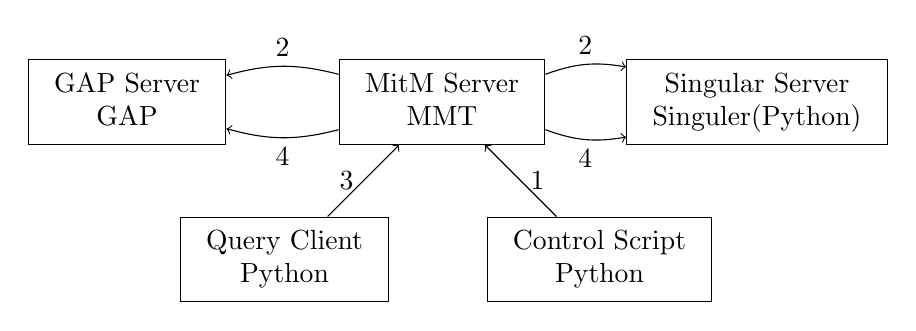
\begin{tikzpicture}[xscale=2, yscale=2]\normalsize
  \node[draw] (g) at (0,0) {
    \begin{tabular}{c}
      GAP Server \\GAP
    \end{tabular}
  };
  \node[draw] (m) at (2,0) {
    \begin{tabular}{c}
      MitM Server\\MMT
    \end{tabular}
  };
  \node[draw] (s) at (4,0) {
    \begin{tabular}{c}
      Singular Server\\Singuler(Python)
    \end{tabular}
  };
  \node[draw] (p) at (1, -1) {
    \begin{tabular}{c}
      Query Client\\Python
    \end{tabular}
  };
  \node[draw] (c) at (3, -1) {
    \begin{tabular}{c}
      Control Script\\Python
    \end{tabular}
    };
  \draw[->] (c) to node[right] {1} (m);
  \draw[->] (m) to[bend left=15] node[above] {2} (s);
  \draw[->] (m) to[bend right=15] node[above] {2} (g);
  \draw[->] (p) to node[left] {3} (m);
  \draw[->] (m) to[bend right=15] node[below] {4} (s);
  \draw[->] (m) to[bend left=15] node[below] {4} (g);
\end{tikzpicture}

%  LocalWords:  tikzpicture xscale yscale Singuler

  \caption[\GAP-\Singular MitM Interaction]{
    System Designed to Prove the Concept of the MitM Protocol
  }\label{fig:mitmpoc}
\end{figure}

The procedure illustrated in figure \ref{fig:mitmpoc} is as follows:
\begin{enumerate}
  \item The control script establishes an \SCSCP connection with the MMT MitM 
    server and aligns the functions exposed by the CAS (\GAP and \Singular) with
    global symbols.
  \item The MitM server establishes \SCSCP connections with the CAS server at
    provided addresses.
  \item The query client queries the MitM server for symbols from public CDs
    without any knowledge of the CAS in operation to calculate orbits of 
    polynomials.
  \item MitM server redirects the requests from the query client to the necessary
    CAS.
\end{enumerate}

\subsection{Components of the Study System}
\subsubsection{MMT MitM Server}
The MitM server is implemented as an MMT-shell extension. The integration into the
MMT ecosystem will be useful in the future for the automation of function 
alignment and type-checking of arguments. It is also queried via \SCSCP as opposed 
to QMT, because currently \SCSCP is more widely supported, e.g. by the \GAP and 
\Python packages.

\subsubsection{\GAP \SCSCP Server}
\GAP server uses the \GAP \SCSCP package to expose the minimal functions needed for 
this study- the constructor for a symmetric group of size N, and a function that
takes a list and a symmetric group and returns a permutation of the list for every 
member of the symmetric group that is obtained by applying that member to every
item of the list.

\subsubsection{\Singular \SCSCP Server}
Since \Singular currently doesn't have any support for \SCSCP, the \Singular \SCSCP server is
written in \Python using the \lstinline|scscp| and \lstinline|PySingular| python modules
and is adapted from the example code on the py-scscp repository\cite{PySCSCP}. The only
function exposed by this server is the evaluation of equality of two applications of the
DMP symbol.

\subsubsection{Controlling Client Script}
In the long term, the function alignment will be done automatically when a CAS 
informs the MitM server of its presence. Currently, however, the export of CAS 
type systems is still a work in progress, so the function alignment is done
via the MitM protocol. The job of the controlling script is thus to align the 
constructor of symmetric group of size N and the orbit of a list to their 
respective symbols in public CDs, as well as registering the ability of the 
\Singular server to equate polynomials.

\subsubsection{Naive Client}
The main client that queries the MitM server has no knowledge of the underlying 
CAS. It follows the procedure:
\begin{enumerate}
  \item Create an OpenMath polynomial.
  \item Obtain a symmetric group of size that is equal to the number of variables 
    in the polynomial from MitM.
  \item Using the obtained group, query MitM for all permutations of the list 
    of variables.
  \item Create polynomials from the permutations of the list of variables.
  \item Filter out the duplicate polynomials by querying MitM for equality of 
    polynomials.
\end{enumerate}
While this is very much a brute-force algorithm to calculate an orbit of a
polynomial, it showcases the ability of the client to query the MitM server that 
is then forced to use multiple CAS without the client needing any knowledge of the
underlying systems.

\subsection{Using the System}
\subsubsection{Dependencies}
The dependencies of the software in subject of the study and instructions on
acquiring them:
\begin{itemize}
  \item \textbf{Jupyter}- installed via pip
  \item \textbf{\GAP}- installed from https://github.com/gap-system/gap
  \item \textbf{\Singular}- installed via package manager or from
    https://www.singular.uni-kl.de/index.php/singular-download.html
  \item \textbf{MMT}- installed from https://github.com/Uniformal/MMT
  \item \textbf{Py-SCSCP}- installed via pip
  \item \textbf{PySingular}- installed via pip or from 
    https://github.com/sebasguts/SingularPython
\end{itemize}

\subsubsection{Execution}
Instructions on running the system:
\begin{itemize}
  \item Run singular\_server.py script using python, the gap\_server.g script
    using \GAP, and start MMT. From the MMT shell prompt, run 
    "file mitm\_server.msl".
  \item Run ControllingClient.py using python to set up alignments between
    MitM server and CAS servers.
  \item Start a Jupyter kernel using "jupyter notebook" and open the 
    QueryingClient.ipynb notebook. This is the example procedure that showcases
    a few examples of calculations of orbits of polynomials.
\end{itemize}

\subsection{Evaluation of the Study}
This study has implemented the MitM approach using \SCSCP, showing that the MitM 
paradigm is an achievable goal. Currently, however, the MitM server acts as 
merely a proxy, redirecting \SCSCP requests to CAS that know how to evaluate them.
For MitM to be a truly modular abstract algebra environment, the following
changes must be made:
\begin{itemize}
  \item A peer-to-peer connection must be made with the CAS servers, so that
    CAS servers can, in turn, query MitM if during a computation they encounter 
    a concept that lies outside their field of knowledge. In application to
    this particular case, it would be cleaner if, instead of asking MitM to 
    produce permutations of a list, the client simply queries MitM for the orbit 
    of a polynomial by defining an action of a member of the symmetric group on a 
    polynomial. \GAP would then be able to calculate the orbit by making the group 
    act on the polynomial with the described action and querying MitM for 
    equality of polynomials, resulting in a linear-time algorithm instead of
    quadratic-time behaviour displayed by the current client.
  \item Alignment between CAS servers and the MitM server must be automated.
    Although manual alignment as described in this case study is usable and
    enables pinpoint alignments to be made, it is not scalable. Any CAS that aims
    to be MitM-compatible should develop a representation of its type system
    in MMT, so that, upon establishing a connection with a new CAS system, the 
    MitM server would be able to automatically align newly accessible functions 
    with symbols from public CDs. This will also enable MMT to act as more than
    a routing proxy, as it would be able to typecheck the arguments of incoming
    requests, making the MitM system more rigid.
\end{itemize}

%%% Local Variables:
%%% mode: latex
%%% TeX-master: "paper"
%%% End:

%  LocalWords:  subsubsection mitm itemize textbf centering fig:mitmpoc lstinline scscp
%  LocalWords:  Jupyter _server.msl ControllingClient.py QueryingClient.ipynb bibitem
%  LocalWords:  thebibliography _server.msl sec:mitm_poc


%%% Local Variables:
%%% mode: latex
%%% TeX-master: "paper"
%%% End:

%  LocalWords:  sec:mitm Jupyter jupyter-project:on KohDavGin:psewads11 BusCapCar:2oms04 standardization DehKohKon:iop16 textbf RabKoh:WSMSML13,uniformal:on MueGauKal:cacfms17 sec:apit serialize normalizer mathcal compute-the-normalizer MitM-based centering mitmcomm MueRoYuRa:abtafs17 Rabe:MAGMS13,uniformal:on inparaenum Sagey lstlisting scscp mmt,is_cyclic scscp lmfdb mmt,query transitivegroup lstinline gap,is_cyclic,scscp lmfdb,query synthesizes mathescape
%  LocalWords:  wrapfigure vspace tikzinput mistargraph fig:mitm mitm_poc
